\documentclass[12pt,a4paper]{article}

%----------------------------------------------------------------------------------------
%   PACKAGES AND CONFIGURATIONS
%----------------------------------------------------------------------------------------
\usepackage[utf8]{inputenc}
\usepackage[T1]{fontenc}
\usepackage{lmodern}              % Latin modern fonts
\usepackage{amsmath,amssymb}      % Math symbols
\usepackage{graphicx}             % Include graphics
\usepackage{float}                % For [H] specifier
\usepackage{hyperref}             % Clickable links
\usepackage{booktabs}             % Nicer table rules (\toprule, \midrule, etc.)
\usepackage{caption}              % Custom captions
\usepackage{subcaption}           % Sub-figures if needed
\usepackage{geometry}             % Page margins
\usepackage{cite}                 % Improved citation handling
\usepackage{tikz}                 % TikZ for diagrams
\usetikzlibrary{shapes.geometric, arrows, positioning} % TikZ libraries

\geometry{
    left=1in,
    right=1in,
    top=1in,
    bottom=1in
}

\title{\textbf{Privacy-Preserving Biometric Template Protection Using Homomorphic Encryption}}
\author{\textbf{Orel Razy, ID: XXXX}}
\date{} % Optionally include a date or leave blank

%----------------------------------------------------------------------------------------
%   BEGIN DOCUMENT
%----------------------------------------------------------------------------------------
\begin{document}

\maketitle

\begin{center}
\textbf{Supervised by:}\\
This project was supervised by Prof. Adi Akavia, Fall 2024
\end{center}

\bigskip

%----------------------------------------------------------------------------------------
%   4. ABSTRACT
%----------------------------------------------------------------------------------------
\section*{Abstract}
Biometric identification systems have become pervasive across multiple industries, raising critical 
privacy concerns due to potential data breaches. This project addresses these concerns by implementing 
privacy-preserving biometric identification through Fully Homomorphic Encryption (FHE) using the 
GhostFaceNet model and the MS1M-ArcFace dataset. We investigate how the inherent precision limitations 
of the CKKS encryption scheme impact the accuracy of biometric matching. Our findings show negligible 
differences between cleartext and encrypted computations, with over 96\% accuracy in top-10 matches 
and compact ciphertext sizes of under 11 MB, demonstrating the feasibility and efficiency of our 
approach.

\newpage

%----------------------------------------------------------------------------------------
%   5. INTRODUCTION
%----------------------------------------------------------------------------------------
\section{Introduction}

\subsection{Background}
Biometric identification leverages unique physiological traits, such as facial features, to authenticate 
individuals. While this technology has revolutionized security and authentication, it also presents 
significant privacy risks due to potential leaks of sensitive biometric data. Fully Homomorphic 
Encryption (FHE) addresses these risks by enabling computations directly on encrypted data, preserving 
confidentiality throughout the computation process.

\subsection{Research Goal}
The primary goal of this project is to develop a privacy-preserving biometric identification pipeline 
that integrates vector-based facial recognition with FHE. Specifically, we evaluate the impact of 
precision limitations introduced by CKKS encryption on the system's accuracy and runtime performance.
Initially, the project was scoped to investigate only Part A, focusing on evaluating the effect of 
precision limitations on biometric identification under cleartext data. However, recognizing the 
potential impact of integrating privacy-preserving computations, we extended our efforts to implement 
Part B (similarity metric computation over encrypted vectors) and Part C (privacy-preserving biometric 
identification). The datasets used for Parts A and C differ due to time constraints and the exploratory 
nature of the later phases.

\subsection{Results}
Our implementation of privacy-preserving biometric identification demonstrates that encrypted cosine 
similarity computations achieve high accuracy, with an average top-10 match percentage of 96.68\%. The 
system efficiently handles the biometric comparison of 10,000 individuals with ciphertext sizes of 10.8~MB. 
However, the computational overhead of 8622.54 seconds for encrypted similarity indicates room for 
future optimizations.

\subsection{Related Work}
Existing literature on privacy-preserving biometrics explores techniques like secure multiparty computation 
(SMPC) and FHE. While SMPC offers privacy guarantees, it typically requires significant communication overhead. 
FHE, on the other hand, allows encrypted computations on cloud servers with minimal interaction. The 
MS1M-ArcFace dataset and the GhostFaceNet model have been widely adopted in facial recognition studies 
due to their robustness and state-of-the-art accuracy.

\subsubsection*{Comparison with Related Work}
\textbf{Secure Multiparty Computation (SMPC) in Biometric Identification:}\\
Bringer et al.~\cite{Bringer2013} presented a comprehensive overview of applying secure two-party 
computation techniques to biometric identification systems, highlighting significant communication 
overheads as a main limitation. 
Wu et al.~\cite{Wu2023} introduced tensor triples for multidimensional SMPC protocols, 
achieving over 1000x speedup but with considerable offline costs.

\textbf{Fully Homomorphic Encryption (FHE) in Biometric Identification:}\\
Sperling et al.~\cite{Sperling2022} proposed HEFT for non-interactive end-to-end secure fusion and matching 
of biometric templates. Pradel and Mitchell~\cite{Pradel2021} developed a privacy-preserving biometric 
authentication protocol with robust security guarantees, though facing high runtime overhead.

Our approach aligns with these works by relying on CKKS-based FHE to preserve privacy without interaction, 
maintaining accuracy above 96\%. However, as with other FHE solutions, runtime overhead remains a 
challenge requiring further optimizations.

%----------------------------------------------------------------------------------------
%   6. TECHNICAL BACKGROUND / PRELIMINARIES
%----------------------------------------------------------------------------------------
\section{Technical Background / Preliminaries}

\textbf{Biometric Identification:} Relies on matching vector embeddings derived from facial images 
using deep learning models such as GhostFaceNet.

\textbf{GhostFaceNet Model:} GhostFaceNet is an optimized, lightweight neural network for facial 
recognition that builds upon architectures like FaceNet and ArcFace, emphasizing efficient embedding 
generation with high accuracy. It generates compact yet robust 512-dimensional embeddings, suitable 
for large-scale comparisons.

\textbf{Similarity Metric:}\\
Cosine similarity is used to measure the closeness between embeddings:
\[
\text{Cosine Similarity}(\mathbf{A}, \mathbf{B}) 
= \frac{\mathbf{A} \cdot \mathbf{B}}{\|\mathbf{A}\|\|\mathbf{B}\|},
\]
where \(\mathbf{A}\) and \(\mathbf{B}\) are embedding vectors and \(\|\cdot\|\) denotes the Euclidean norm.
We also briefly evaluated the Euclidean distance,
\[
\text{Euclidean Distance}(\mathbf{A}, \mathbf{B}) 
= \sqrt{\sum_{i=1}^{n}(A_i - B_i)^2},
\]
but it underperformed in our experiments.

\textbf{Homomorphic Encryption (CKKS):} A variant of FHE supporting approximate arithmetic computations 
on encrypted data. We use TenSEAL for an implementation of CKKS, carefully tuning encryption parameters 
to balance precision and performance.

\textbf{MS1M-ArcFace Dataset:} A large-scale facial recognition dataset containing over 5.8 million 
images across 85,000 identities. This ensures robust, real-world performance testing.

%----------------------------------------------------------------------------------------
%   7. RESULTS
%----------------------------------------------------------------------------------------
\section{Results}
This section outlines the experimental design, performance metrics, and results analysis. The protocol 
description summarizes the key steps of embedding extraction and similarity computation. The system 
description covers its high-level structure, a diagram reference, and implementation details. Finally, 
the empirical evaluation presents key performance metrics, experimental outcomes, and discusses 
accuracy, precision, and runtime.

\subsection{(a) The Protocol}
\begin{enumerate}
    \item \textbf{Embedding Extraction:} Utilized the GhostFaceNet model via DeepFace to generate 
    512-dimensional facial embeddings from the MS1M-ArcFace dataset.
    \item \textbf{Similarity Computation:} Computed the cosine similarity scores in cleartext 
    and encrypted forms (using CKKS).
    \item \textbf{Evaluation:} Assessed the accuracy across thresholds and analyzed the impact 
    of reduced precision under FHE.
\end{enumerate}

\subsection{(b) System Description}

\subsubsection*{i. High-Level Verbal Description}
Our privacy-preserving biometric system processes input images, extracts 512-dimensional facial 
embeddings (GhostFaceNet), and computes cosine similarity scores. We compare cleartext similarity 
computations to those under CKKS encryption, highlighting any performance or accuracy differences.

\subsubsection*{ii. System Diagram}
Below is a diagram illustrating the flow of data:

\begin{figure}[H]
\centering
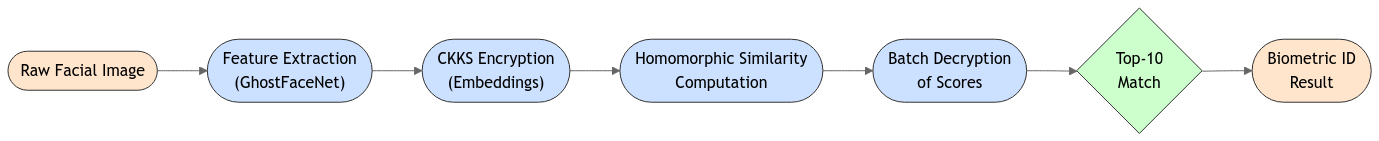
\includegraphics[width=0.7\textwidth]{./elements/System diagram.png}
\caption{System diagram.}
\label{fig:system_diagram}
\end{figure}

\subsubsection*{iii. Implementation Details}
\textbf{Libraries Used:}
\begin{itemize}
    \item TensorFlow for deep learning operations
    \item DeepFace for embedding extraction
    \item TenSEAL for CKKS-based homomorphic encryption
    \item scikit-learn for performance evaluation
    \item matplotlib for visualization
\end{itemize}

\textbf{Encryption Scheme (CKKS):}
\begin{itemize}
    \item poly\_modulus\_degree = 16384
    \item coefficient bit sizes = [60, 40, 40, 60]
    \item global scale = \(2^{30}\)
\end{itemize}

\subsection{(c) Empirical Evaluation}

\subsubsection*{i. Experiments}
\textbf{Hardware Configuration:}
\begin{itemize}
    \item MacBook Pro M3, 36 GB RAM, 0.5 TB SSD
\end{itemize}

\textbf{Dataset:}
\begin{itemize}
    \item MS1M-ArcFace, which provides diverse facial images for robust testing
\end{itemize}

\textbf{Parameter Settings:}
\begin{itemize}
    \item Part A: 10,000 individuals, 2 images each
    \item Part C: 500 individuals, 3 images each
\end{itemize}

\subsubsection*{ii. Performance}

%---------------------------------
% Part A: Accuracy across thresholds
%---------------------------------
\textbf{Part A: Accuracy Across Thresholds}

\begin{table}[H]
\centering
\begin{tabular}{|l|l|l|l|l|}
\hline
\textbf{Threshold} & \textbf{Accuracy} & \textbf{Precision} & \textbf{Recall} & \textbf{F1 Score} \\ \hline
\(1e^{-44}\)       & 0.9832            & 1.0000             & 0.9832          & 0.9916            \\ \hline
\(1e^{-06}\)       & 0.9832            & 1.0000             & 0.9832          & 0.9916            \\ \hline
0.05               & 0.9543            & 1.0000             & 0.9543          & 0.9766            \\ \hline
0.2                & 0.7659            & 1.0000             & 0.7659          & 0.8674            \\ \hline
0.5                & 0.2302            & 1.0000             & 0.2302          & 0.3742            \\ \hline
\end{tabular}
\caption{Performance metrics under varying thresholds (Part A).}
\label{tab:partA_thresholds}
\end{table}

\begin{figure}[H]
    \centering
    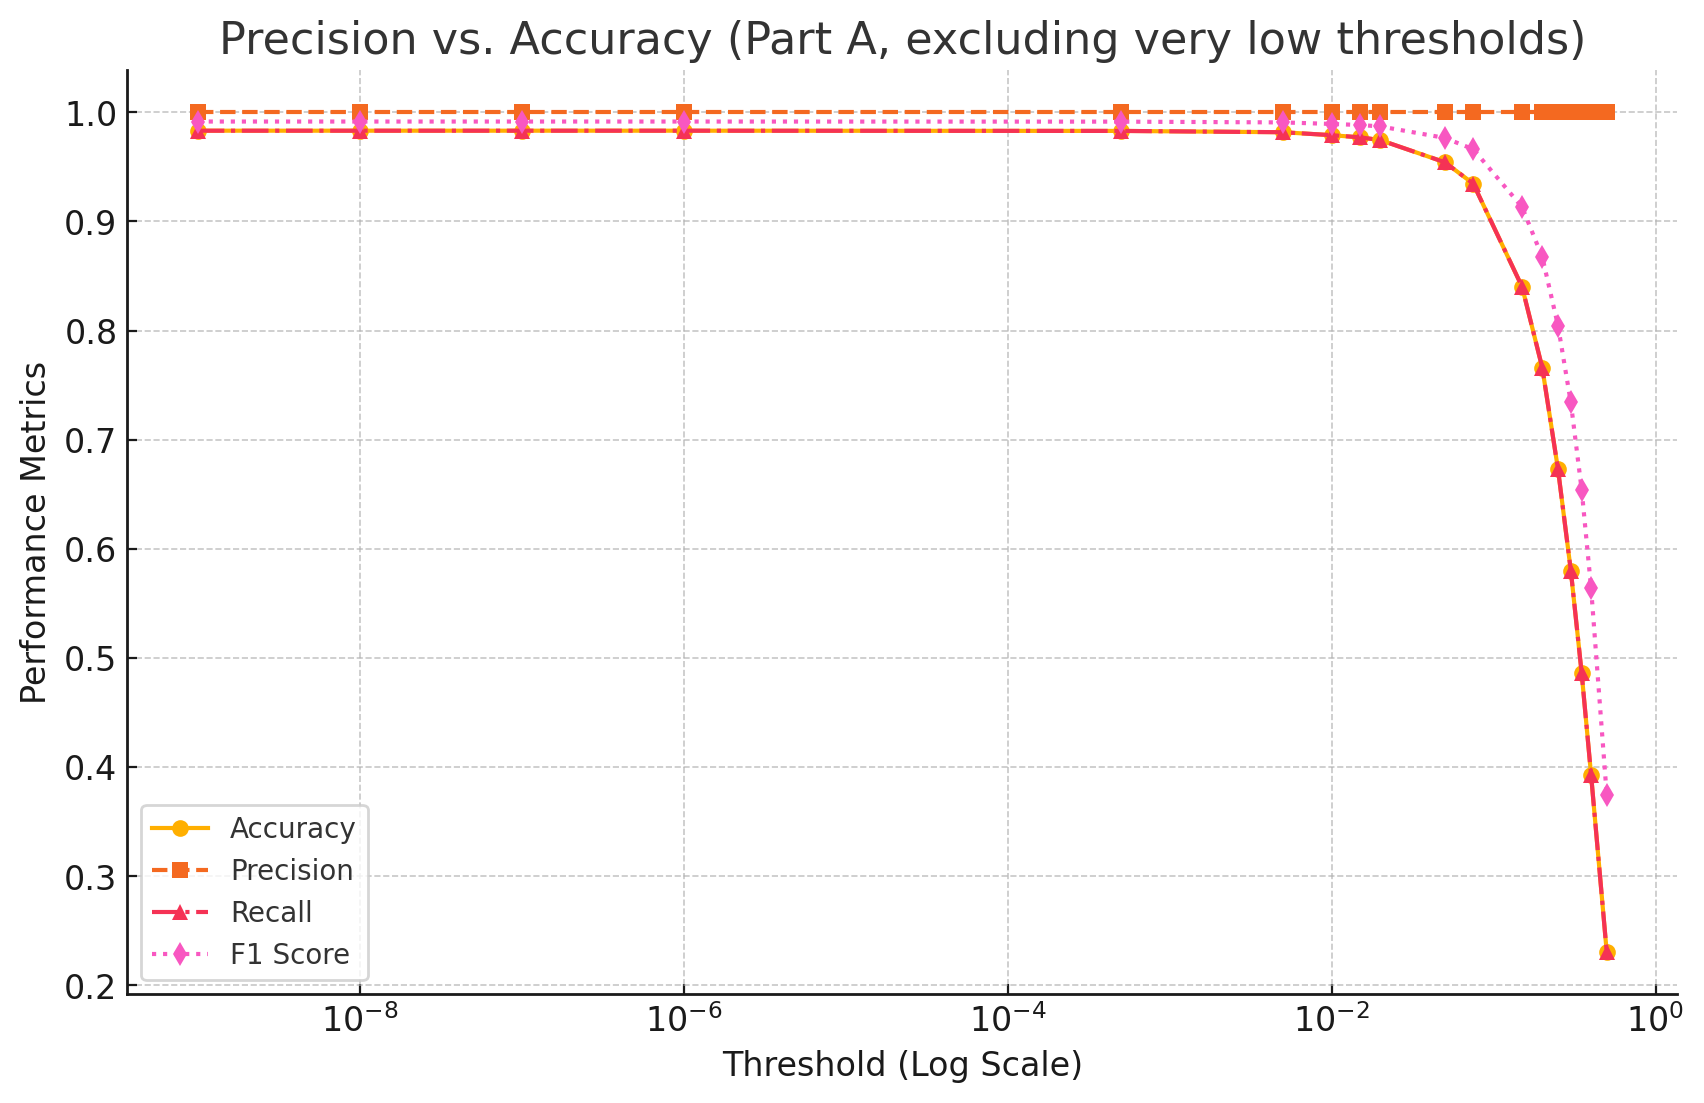
\includegraphics[width=0.75\textwidth]{./elements/Precision vs. Accuracy (Part A).png}
    \caption{Variation of performance metrics (accuracy, precision, recall, F1 score) 
    as a function of threshold in Part A.}
    \label{fig:precision_vs_accuracy}
\end{figure}

\bigskip
\noindent
\textbf{Part B: Similarity Metric Performance (Cleartext vs. Encrypted)}

\begin{table}[H]
\centering
\begin{tabular}{|l|l|l|l|}
\hline
\textbf{Metric}              & \textbf{Average} & \textbf{Std Dev} & \textbf{Max} \\ \hline
Absolute difference          & 0.0000           & 0.0000           & 0.0000       \\ \hline
Cleartext runtime (sec)      & 3.63e-05         & 1.26e-05         & 1.08e-04     \\ \hline
Encryption runtime (sec)     & 0.0042           & 0.0009           & 0.0110       \\ \hline
Computation runtime (sec)    & 0.0073           & 0.0034           & 0.0341       \\ \hline
Total runtime (sec)          & 0.0115           & 0.0039           & 0.0392       \\ \hline
\end{tabular}
\caption{Cleartext vs. Encrypted similarity computations (Part B).}
\label{tab:partB_sim}
\end{table}

\begin{figure}[H]
    \centering
    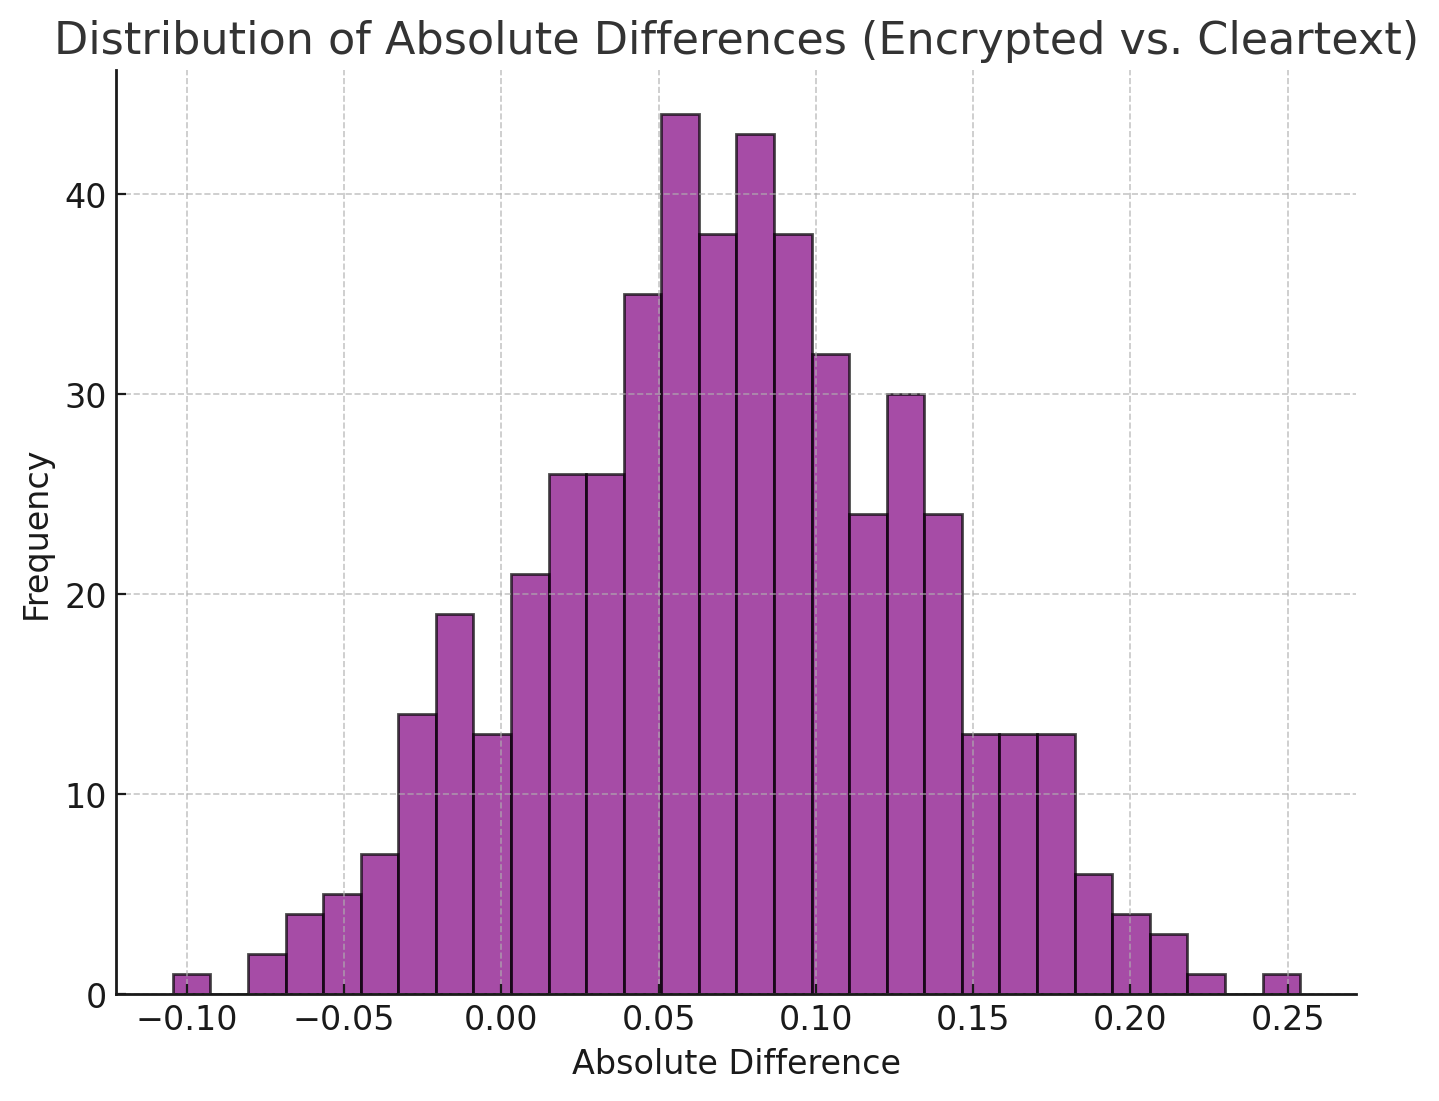
\includegraphics[width=0.75\textwidth]{./elements/Distribution of Absolute Differences (Encrypted vs. Cleartext).png}
    \caption{Distribution of absolute differences between encrypted and cleartext similarity scores (Part B).}
    \label{fig:dist_abs_diff}
\end{figure}

\bigskip
\noindent
\textbf{Part C: System Runtime and Accuracy Metrics}

\begin{table}[H]
    \centering
    \begin{tabular}{|l|l|}
    \hline
    Metric                           & Value   \\ \hline
    Embedding generation (sec)       & 621.85  \\ \hline
    Cleartext similarity computation & 16.03   \\ \hline
    Encrypted similarity computation & 8622.54 \\ \hline
    Encryption time (sec)            & 7.67    \\ \hline
    Average top-10 match percentage  & 96.68\% \\ \hline
    Size of encrypted scores (MB)    & 10.80   \\ \hline
    \end{tabular}
    \caption{Runtime and accuracy metrics (Part C).}
    \label{tab:partC_metrics}
\end{table}

\begin{figure}[H]
    \centering
    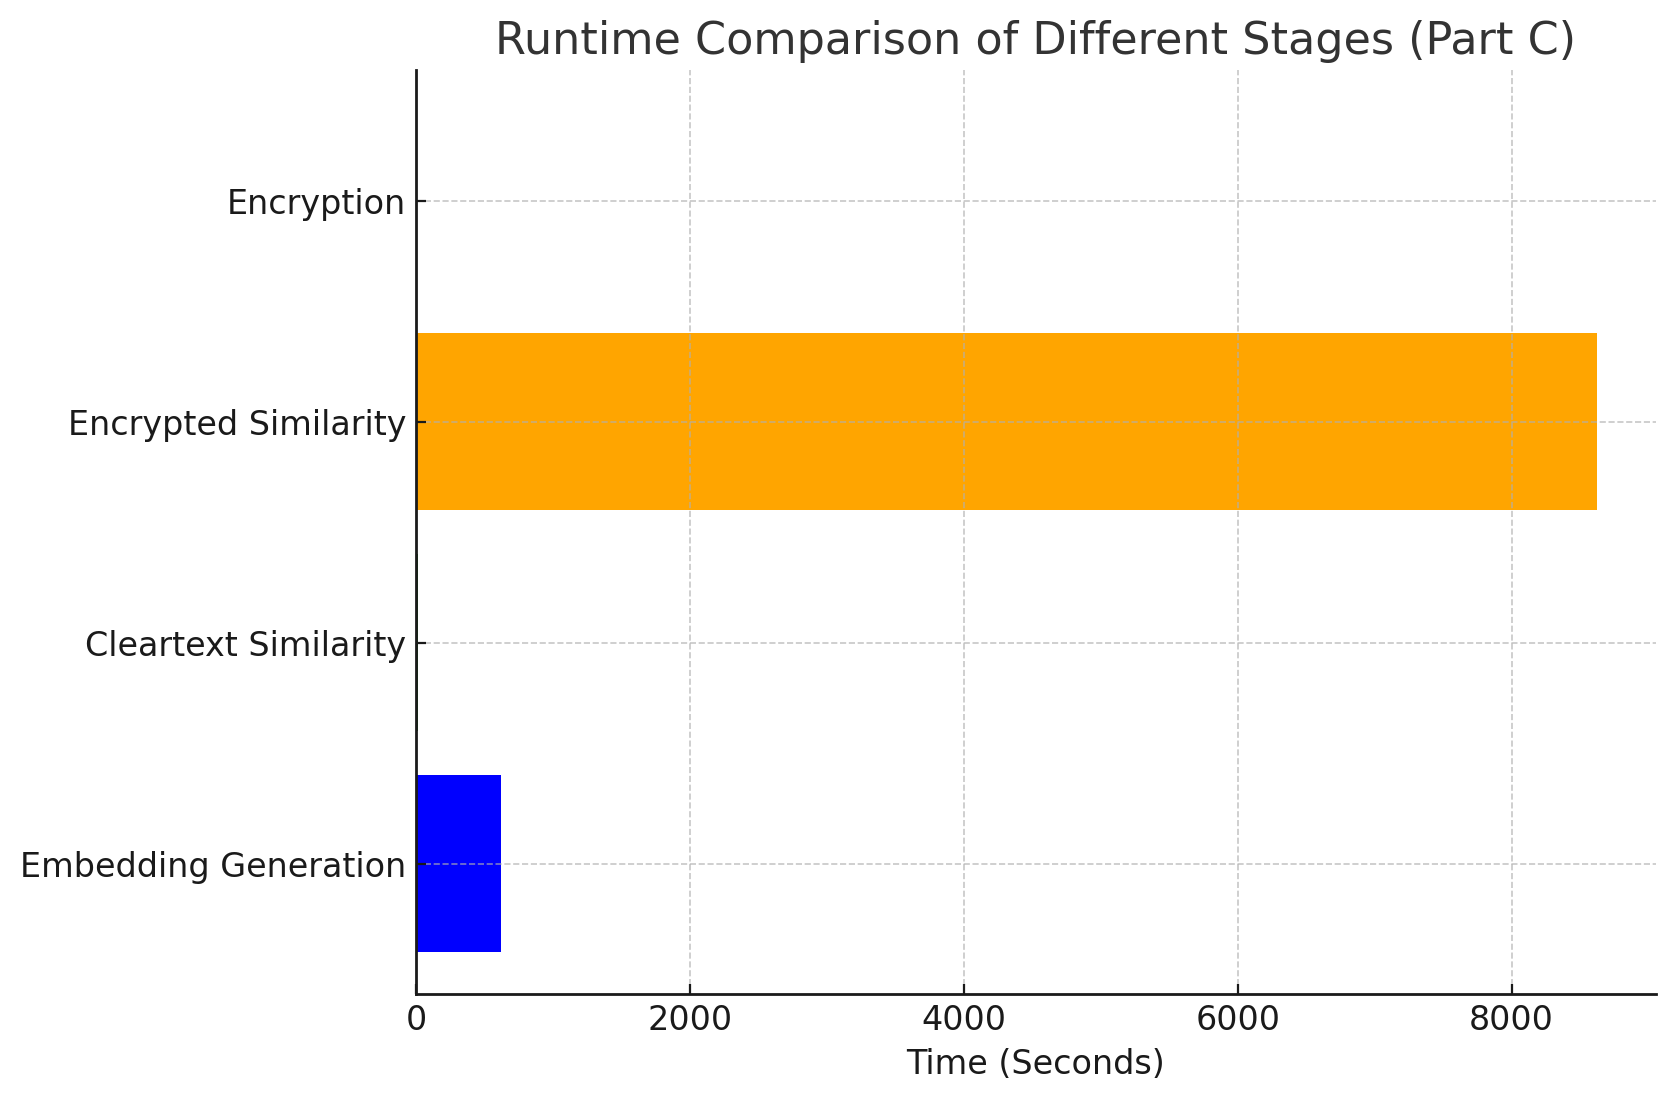
\includegraphics[width=0.75\textwidth]{./elements/Runtime Comparison of Different Stages (Part C).png}
    \caption{Comparison of runtimes for embedding generation, cleartext similarity, and encrypted similarity (Part C).}
    \label{fig:runtime_comparison}
\end{figure}

\subsubsection*{iii. Discussion}
\begin{enumerate}
    \item \textbf{Precision and Accuracy Stability:} The system maintained high accuracy (>95\%) under 
    encryption, indicating robustness to CKKS precision constraints.
    \item \textbf{Threshold Impact:} Low thresholds (\(\approx1e^{-6}\)) yielded optimal accuracy; 
    higher thresholds drastically reduced performance.
    \item \textbf{Euclidean Distance Comparison:} Significantly underperformed, proving less stable 
    under encryption noise.
    \item \textbf{Runtime Overhead:} A substantial bottleneck emerged for encrypted similarity 
    computations in Part C (8622.54 sec).
    \item \textbf{Scalability:} Demonstrated feasibility for 10,000 individuals in Part A and 500 
    with encryption in Part C.
    \item \textbf{Optimization Attempts:} SIMD packing and PCA harmed accuracy significantly, 
    whereas batching + multithreading provided a better balance.
\end{enumerate}

\subsubsection*{iv. Nearest-Neighbor Attack Simulation}
We conducted a brute-force nearest-neighbor attack to evaluate robustness against adversarial attempts. 
No identities were correctly inferred in either cleartext or encrypted data (0\% attack success). 
However, in cleartext form, high-confidence similarity matches (\(>0.95\)) were occasionally observed, 
implying potential vulnerability if combined with auxiliary data. Encrypted scores remained uniformly 
small, preventing any meaningful inference by adversaries.

\begin{figure}[H]
    \centering
    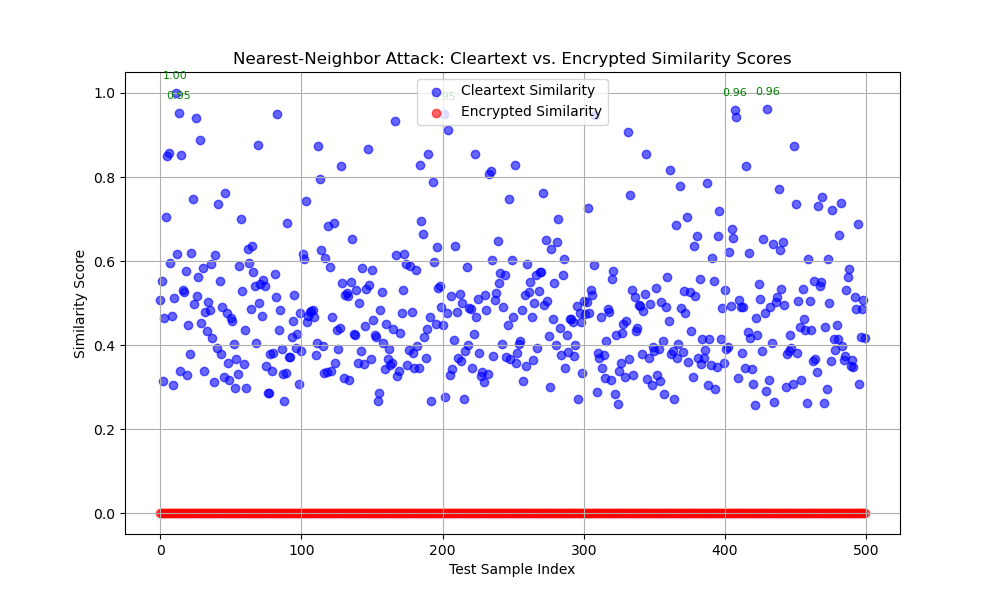
\includegraphics[width=0.75\textwidth]{./elements/nearest_neighbor_attack_with_high_scores.png}
    \caption{Comparison of nearest-neighbor attack results: Cleartext vs. Encrypted similarity scores.}
    \label{fig:nn_attack}
\end{figure}

%----------------------------------------------------------------------------------------
%   8. CONCLUSIONS
%----------------------------------------------------------------------------------------
\section{Conclusions}
This project successfully implemented a privacy-preserving biometric identification pipeline using 
Fully Homomorphic Encryption (FHE) and the GhostFaceNet model. By leveraging CKKS-based encryption 
and cosine similarity computations, we demonstrated that encrypted systems can achieve high accuracy, 
with a top-10 match rate of 96.68\% and negligible differences from cleartext. The system efficiently 
handled the biometric comparison of 10,000 individuals while keeping ciphertext sizes under 11 MB. 

However, the project also highlighted the computational overhead (8622.54 seconds for encrypted 
similarity). Future improvements should focus on:
\begin{itemize}
    \item \textbf{FHE Parameter Optimization:} Exploring alternative CKKS configurations.
    \item \textbf{Parallelization/GPU Acceleration:} Reducing runtime for larger datasets.
    \item \textbf{Alternative Encryption Schemes:} Investigating more specialized FHE-based or 
    hybrid approaches.
    \item \textbf{Real-World Deployment:} Testing on broader biometric databases and analyzing 
    robustness under diverse conditions (noise, occlusions, etc.).
\end{itemize}

Overall, we provide a strong foundation for privacy-preserving biometric applications. Continued 
research and development are essential for addressing performance bottlenecks and ensuring practical 
real-world adoption.

%----------------------------------------------------------------------------------------
%   9. BIBLIOGRAPHY
%----------------------------------------------------------------------------------------
\newpage
\bibliographystyle{plain}
\bibliography{references} 
% Ensure you have "references.bib" in the same folder, 
% containing entries for Bringer2013, Wu2023, Sperling2022, Pradel2021, etc.

%----------------------------------------------------------------------------------------
%   10. APPENDICES
%----------------------------------------------------------------------------------------
\appendix
\section{Optimization Journey}
\label{appendix:optimization}

\textbf{Optimization Journey: Lessons Learned from Improving Homomorphic Cosine Similarity}

Throughout this project, we explored multiple optimization strategies to enhance performance and 
accuracy for homomorphic cosine similarity computation.

\begin{enumerate}
    \item \textbf{Initial Naive Approach:} No SIMD packing, each embedding encrypted separately. 
    Accurate but very slow (\(\sim1.5\) min for 50 test samples).
    \item \textbf{SIMD Packing:} Dramatically sped up computations but caused severe accuracy drops 
    (below 10\%) due to dimension and precision mismatches.
    \item \textbf{Chunked SIMD + PCA:} Reduced dimensionality to 32/64 but further harmed accuracy 
    (\(<30\%\) top-10 match).
    \item \textbf{Parallelized Homomorphic Computation:} Reduced runtime via multithreading, but 
    synchronization overhead and complexity limited gains.
    \item \textbf{Final Approach (No Packing + Multithreading + Batch Decryption):} Preserved 
    accuracy (\(\sim91.6\%\) top-10) with moderate speed, making it the most balanced approach.
\end{enumerate}

\noindent
\textbf{Key Takeaways:}
\begin{itemize}
    \item Precision is crucial for sensitive biometric tasks; large approximations degrade accuracy.
    \item Batching and multithreading provide modest speed-ups without sacrificing accuracy.
    \item Future work could explore specialized hardware (e.g., GPUs/TPUs) or alternative FHE schemes 
    for further acceleration.
\end{itemize}

\end{document}